% 0153(본책 27쪽) — x절편 6, y절편 −8 인 직선의 그래프. 스캔 그림이라 TikZ 로 다시 그림.
% 라벨은 원문 그대로 O·x·y 와 눈금 6·−8 만. 직선의 식은 적지 않는다.
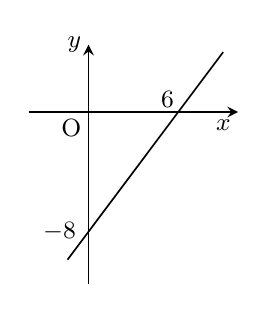
\begin{tikzpicture}[scale=0.19, line width=0.5pt]
  \draw[->, >=stealth, line width=0.7pt] (-4,0) -- (10,0) node[below left=-1pt, font=\small] {$x$};
  \draw[->, >=stealth, line width=0.7pt] (0,-11.5) -- (0,4.5) node[left=-1pt, font=\small] {$y$};
  \draw[line width=0.6pt] (-1.4,-9.87) -- (9,4);
  \node[below left=-1pt, font=\small] at (0,0) {$\mathrm{O}$};
  \node[above left=-2pt, font=\small] at (6,0) {$6$};
  \node[left=1pt, font=\small] at (0,-8) {$-8$};
\end{tikzpicture}
